\documentclass[11pt,a4paper]{article}
\usepackage[margin=0.75in]{geometry}
\usepackage{graphicx}
\usepackage{amsmath}
\usepackage{hyperref}
\usepackage{tikz}
\usepackage{enumitem}
\usepackage{booktabs}
\usepackage{array}
\usetikzlibrary{shapes.geometric, arrows.meta, positioning, fit, backgrounds, calc}
\title{\textbf{Project Synopsis: Operating Systems Lab}\\[0.3em]\large toyOS: A Miniature Operating System in User Space}
\author{}
\date{}
\begin{document}
\maketitle
\vspace{-3.5em}
\noindent\textbf{Batch:} B5 \hfill \textbf{Department:} CSE \& IT, JIIT
\vspace{0.5em}

\noindent\textbf{Team Members:} \hfill \textbf{Submitted To:}
\begin{itemize}[leftmargin=*, itemsep=0pt, parsep=0pt, topsep=0pt]
    \item Harsh Sharma (2401030232) \hfill Dr. Prakash Kumar
    \item Karvy Singh (2401030234) \hfill Dr. Vikash
    \item Rudra Kumar Singh (2401030237) \hfill Ms. Sonal Saurabh
\end{itemize}

\section*{Project Description}
Most lab programs study one OS concept at a time, for example a CPU scheduling program that prints a Gantt chart from a fixed table of burst times. In a real operating system, however, these parts work \emph{together}: the CPU scheduler decides which process runs, that process asks the disk for data, the disk requests are scheduled, memory is shared, and semaphores keep everything consistent.

In this project we build \textbf{toyOS}, a small working operating system that runs as a normal program on Linux, written in C. It has its own \textbf{shell}, \textbf{CPU scheduler}, \textbf{memory manager}, \textbf{disk scheduler}, \textbf{file system} and \textbf{synchronization tools}. The user types commands in the toyOS shell, each command runs as a job (process) inside toyOS, and all the parts of the OS can be watched working together live.

\subsection*{Key Features}
\begin{itemize}[leftmargin=*, itemsep=2pt]
    \item \textbf{Shell:} Commands such as \texttt{ls}, \texttt{cat}, \texttt{cp}, \texttt{rm}, background jobs with \texttt{\&}, and pipes between jobs (\mbox{\texttt{cat a | wc}}).
    \item \textbf{Process management:} Every job has a Process Control Block (PCB) and moves through the states New, Ready, Running, Blocked and Terminated. The \texttt{ps} command shows these states live.
    \item \textbf{CPU scheduling:} FCFS, Round Robin, Priority, SJF and Multilevel Feedback Queue, switchable at runtime. Jobs are actually paused and resumed by our scheduler (real context switches using a timer interrupt). SJF predicts burst times using exponential averaging: $\tau_{n+1} = \alpha\, t_n + (1-\alpha)\,\tau_n$.
    \item \textbf{Memory management:} Memory for each job is allocated from a fixed block of ``RAM'' using First-Fit, Best-Fit or Worst-Fit, and fragmentation is displayed. Disk blocks are kept in a page cache of fixed size, with FIFO, LRU and Clock page replacement; page faults and hit ratio are reported.
    \item \textbf{Disk scheduling:} The disk is a file (\texttt{disk.img}) controlled by a separate disk thread. When several jobs read files at the same time, their requests are ordered using FCFS, SSTF, SCAN or C-LOOK, and total head movement is measured.
    \item \textbf{File system:} A simple file system inside \texttt{disk.img} with a superblock, free-block bitmap, inodes and a directory. Files remain saved between runs.
    \item \textbf{Synchronization:} Our own counting and binary semaphores. Pipes are implemented as the \emph{Producer--Consumer (bounded buffer)} problem, and file access uses the \emph{Readers--Writers} solution. POSIX mutexes and condition variables are used between jobs and the disk thread.
    \item \textbf{Deadlock detection:} A \texttt{deadlock} command builds the wait-for graph of jobs and semaphores and reports any cycle.
    \item \textbf{Statistics:} Gantt chart, average waiting and turnaround time, context switches, page faults and disk head movement, so different algorithms can be compared on the same workload.
\end{itemize}

\section*{System Architecture}
\begin{center}
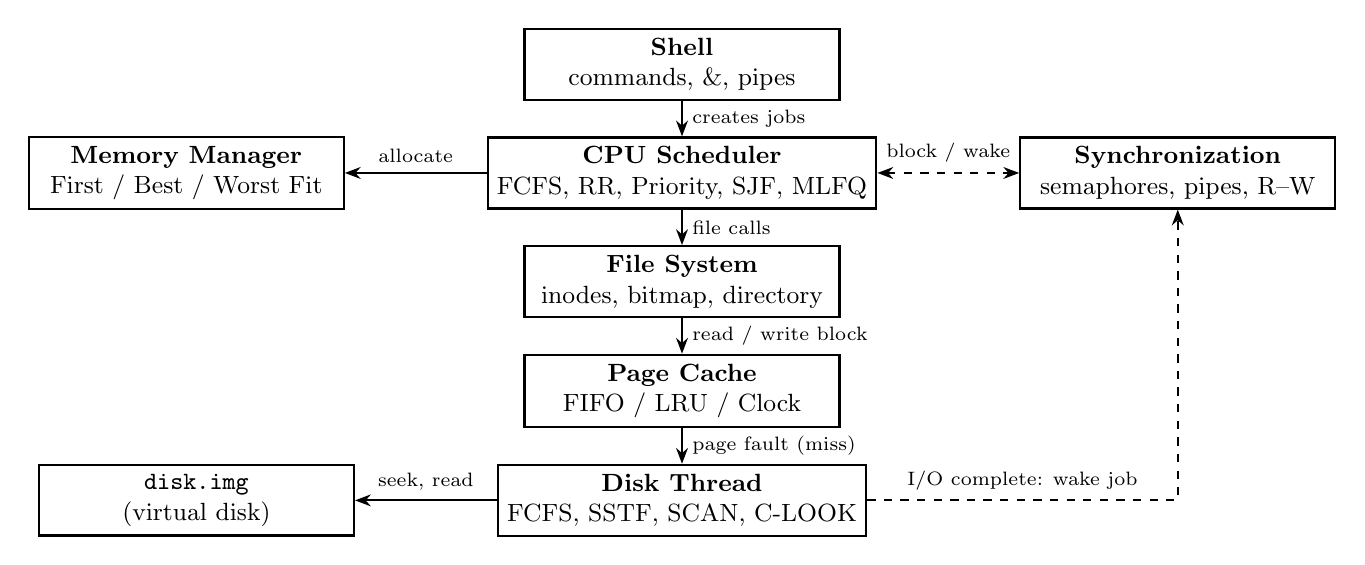
\begin{tikzpicture}[
    box/.style={rectangle, draw=black, thick, minimum width=4.0cm, minimum height=0.85cm, align=center, font=\small},
    arrow/.style={-{Stealth[length=2mm]}, thick},
    lbl/.style={font=\scriptsize}
]
\node[box] (shell) {\textbf{Shell}\\commands, \&, pipes};
\node[box, below=0.45cm of shell] (sched) {\textbf{CPU Scheduler}\\FCFS, RR, Priority, SJF, MLFQ};
\node[box, left=1.8cm of sched] (mem) {\textbf{Memory Manager}\\First / Best / Worst Fit};
\node[box, right=1.8cm of sched] (sync) {\textbf{Synchronization}\\semaphores, pipes, R--W};
\node[box, below=0.45cm of sched] (fs) {\textbf{File System}\\inodes, bitmap, directory};
\node[box, below=0.45cm of fs] (cache) {\textbf{Page Cache}\\FIFO / LRU / Clock};
\node[box, below=0.45cm of cache] (disk) {\textbf{Disk Thread}\\FCFS, SSTF, SCAN, C-LOOK};
\node[box, left=1.8cm of disk] (img) {\texttt{disk.img}\\(virtual disk)};

\draw[arrow] (shell) -- node[right, lbl]{creates jobs} (sched);
\draw[arrow] (sched) -- node[above, lbl]{allocate} (mem);
\draw[arrow, dashed, {Stealth[length=2mm]}-{Stealth[length=2mm]}] (sched) -- node[above, lbl]{block / wake} (sync);
\draw[arrow] (sched) -- node[right, lbl]{file calls} (fs);
\draw[arrow] (fs) -- node[right, lbl]{read / write block} (cache);
\draw[arrow] (cache) -- node[right, lbl]{page fault (miss)} (disk);
\draw[arrow] (disk) -- node[above, lbl]{seek, read} (img);
\draw[arrow, dashed] (disk.east) -| node[pos=0.25, above, lbl]{I/O complete: wake job} (sync.south);
\end{tikzpicture}
\end{center}

\noindent\textbf{Example flow:} running \texttt{cat notes.txt \&} creates a job (\emph{New $\rightarrow$ Ready}). When the scheduler runs it, it asks the file system for a block; if the block is not in the page cache (a page fault), a request goes to the disk queue and the job becomes \emph{Blocked}. The disk thread serves requests in SCAN order and, on completion, wakes the job (\emph{Blocked $\rightarrow$ Ready}), just like an I/O interrupt in a real OS.

\section*{Mapping to Course Syllabus}
\begin{center}
\small
\begin{tabular}{@{}>{\raggedright}p{5.2cm} p{11.0cm}@{}}
\toprule
\textbf{Module} & \textbf{Where it appears in toyOS} \\
\midrule
1. Linux \& Shell & toyOS shell: parsing, built-in commands, background jobs, pipes \\
2. Process Management \& IPC & PCB, process states, \texttt{ps}; pipes between jobs for communication \\
3. Multithreading (pthreads) & Jobs as threads with their own stacks; disk controller as a POSIX thread \\
4. CPU Scheduling & FCFS, RR, Priority, SJF, MLFQ with Gantt chart and timing statistics \\
5. Process Synchronization & Semaphores, binary semaphores, bounded buffer, readers--writers \\
6. Deadlock Management & Wait-for graph and cycle detection with the \texttt{deadlock} command \\
7. Memory Management & First/Best/Worst-Fit allocation; FIFO, LRU, Clock page replacement \\
8. Storage Management & FCFS, SSTF, SCAN, C-LOOK disk scheduling; inode-based file system \\
\bottomrule
\end{tabular}
\end{center}

\section*{Tools \& Technologies}
\textbf{Language:} C (about 1000 lines of code), GCC on Linux. \textbf{System features used:} \texttt{ucontext} (context switching), \texttt{setitimer} and signals (timer interrupt), POSIX threads, mutexes and condition variables, and file I/O on \texttt{disk.img}.

\section*{Expected Outcomes}
\begin{itemize}[leftmargin=*, itemsep=1pt]
    \item A working mini operating system with an interactive shell, in which all OS components work together
    \item Comparison of CPU scheduling algorithms on the same jobs (waiting time, turnaround time, context switches)
    \item Comparison of page replacement (page faults, hit ratio), allocation methods (fragmentation) and disk scheduling algorithms (total head movement)
    \item Practical demonstration of semaphores, classical synchronization problems and deadlock detection
\end{itemize}

\end{document}
